\documentclass[11pt]{article}
\usepackage[margin=1in]{geometry}
\usepackage{amsmath,amssymb}
\usepackage{amsthm}
\usepackage{booktabs}
\usepackage[hidelinks]{hyperref}

\newtheorem{assumption}{Assumption}
\newtheorem{noteenv}{Note}
\newtheorem{problem}{Problem}

% Notation and conventions matching paper.tex
% Symbols: y(t) measured EEG, s(t) neural signal, d_r(t) repetitive disturbance,
% n(t) noise, t_k R-peak instant, T_k beat interval, phi(t) cardiac phase in [0,1)

\title{ECG Phase Estimator for Cardiac Artifact Removal}
\author{Extracted from: Cardiac Field Artifact Removal in Ear-EEG Using Repetitive Disturbance Rejection}
\date{}

\begin{document}

\maketitle

% =========================================================================
% Background: Problem Formulation (excerpted)
% =========================================================================

\section*{Problem Formulation (Background)}

Following repetitive-control modeling conventions, the measured ear-EEG signal is modeled as
\begin{equation}
y(t) = s(t) + d_r(t) + n(t),
\label{eq:meas}
\end{equation}
where $s(t)$ is the neural signal of interest, $d_r(t)$ is the heartbeat-synchronous repetitive 
cardiac disturbance, and $n(t)$ aggregates asynchronous interference and sensor noise. The subscript 
$r$ denotes the repetitive nature of the disturbance. Its period is heartbeat dependent and is set by 
ECG R-peak timing, with beat interval
\begin{equation}
T_k = t_{k+1} - t_k,
\label{eq:Tk}
\end{equation}
where $t_k$ is the $k$-th detected R-peak instant.

\begin{assumption}\label{asm:tk_slowly_varying}
The beat period $T_k$ is assumed slowly varying, dominated by respiratory sinus arrhythmia (RSA), with
additional small modulation from low-level muscle/motion effects in resting-state recordings.
\end{assumption}

The repetitive disturbance is represented as a phase-indexed waveform
\begin{equation}
d_r(t) = d_r\!\left(\phi(t)\right), \qquad
\phi(t) = \frac{t - t_k}{T_k}, \quad t \in [t_k, t_{k+1}),
\label{eq:phase_model}
\end{equation}
with $\phi(t)\in[0,1)$ the R-peak-aligned cardiac phase.

\begin{problem}\label{prob:timing_estimation}
Estimate $\hat{t}_k$ robustly so that EEG samples can be phase-aligned via the phase model.
The estimated cardiac phase between beats advances as
\begin{equation}
\hat{\phi}(t) = \frac{t - \hat{t}_k}{\hat{T}_k}, \qquad \hat{T}_k = \hat{t}_{k+1} - \hat{t}_k,
\label{eq:phi_hat}
\end{equation}
where $\hat{T}_k$ is the estimated beat period.
\end{problem}

\begin{noteenv}\label{note:pll_prediction}
Since $T_k$ is slowly varying (Assumption~\ref{asm:tk_slowly_varying}), $\hat{T}_k$ can be reliably
predicted between successive R-peaks. The PI tracker advances phase continuously between beats so
that $\hat{\phi}(t)$ remains well-defined in real-time causal operation.
\end{noteenv}

% =========================================================================
% Main Section IV Content
% =========================================================================

\section{ECG Phase Estimator}
\label{sec:ecg_phase_estimator}

\subsection{Min/max tracker + PI/PID phase tracking}

A QRS-emphasis band-pass feeds two streaming trackers: a peak tracker $pk(t)$ (fast attack, slow 
release) and a baseline tracker $bl(t)$ (slow moving average). The normalized gate
\begin{equation}
g(t) = \frac{x(t) - bl(t)}{pk(t) - bl(t)}
\label{eq:gate}
\end{equation}
is amplitude-drift invariant, so posture/contact drift does not defeat detection. A Schmitt 
hysteresis and a 250~ms refractory yield clean beat gating; the fiducial $t_k$ is the raw-reference 
maximum within the gated window (low jitter).

A PI phase-locked loop converts sparse fiducials into a continuous phase. Between beats the phase 
advances by the instantaneous rate estimate,
\begin{equation}
p(t+1) = \big[\, p(t) + \mathrm{fr}(t) \,\big] \bmod 1, \qquad \mathrm{fr}(t) = 
\frac{1}{\mathrm{RR}_{\mathrm{est}}(t)\, f_s},
\label{eq:phaseacc}
\end{equation}
where $f_s$ is the sample rate. At each fiducial, a proportional term realigns phase and an 
integral term updates the rate estimate,
\begin{align}
p &\leftarrow p - K_p \, e_p, \label{eq:pcorr}\\
\mathrm{RR}_{\mathrm{est}} &\leftarrow \mathrm{RR}_{\mathrm{est}} + K_i 
\,(\mathrm{RR}_{\mathrm{meas}} - \mathrm{RR}_{\mathrm{est}}), \label{eq:rcorr}
\end{align}
with $e_p$ the wrapped phase error and $K_p,K_i$ the PI gains. The loop bandwidth is set above 
respiratory sinus arrhythmia (RSA, $\sim$0.2--0.4~Hz) and below per-beat detection noise. An 
arrhythmia supervisor classifies each beat by the ratio 
$\mathrm{RR}_{\mathrm{meas}}/\mathrm{RR}_{\mathrm{est}}$ and applies the matching 
reflex---\emph{premature}: trust the measured phase, freeze the rate and learning; \emph{missed}: 
trust the prediction, keep the rate---protecting both the loop and the template.

\subsection{Algorithm summary}

Per sample: (1)~update trackers \eqref{eq:gate} and gate; (2)~advance phase \eqref{eq:phaseacc}, 
correct at fiducials \eqref{eq:pcorr}--\eqref{eq:rcorr}, run the supervisor; (3)~ILC
lookup, limited subtraction, and template update on normal beats. The proposed online path is
therefore constant-time per sample, with template memory 
linear in the window length.

% =========================================================================
% Complexity Analysis (follows immediately after)
% =========================================================================

\section{Complexity Analysis}
\label{sec:complexity_analysis}

Let $L_w$ be the template length and $C$ the channel count. The proposed phase-tracker + ILC path 
is lightweight: tracker updates and gating are constant-time, PI/PID phase update is constant-time 
(amortized), and ILC lookup/update is constant-time with memory $L_w$. Thus, per-sample complexity 
is $O(1)$ and memory is $O(L_w)$ for each channel. This profile is suitable for always-on 
low-power ear-EEG devices. For fairness, baseline adaptive cancellers (e.g., LMS/RLS) are reported 
separately in experiments and are not part of the proposed online deployment path.


\section{Experiments}
\label{sec:experiments}



\subsection{Real ear-EEG validation: coherence and repeatable-template evidence}
\label{sec:realdata}
To test the coherence assumption behind reference-driven cancellers and confirm that a genuine
repeatable cardiac template exists outside simulation, we analyze a 10-minute segment (717 beats;
2 premature, 0 missed) from the SeizeIT2 dataset \cite{seizeit2}, which pairs a wearable
behind-the-ear EEG channel (256~Hz) with a synchronized chest ECG lead during video-EEG epilepsy
monitoring.

\emph{Coherence is near zero, even under best-case R-locked pooling.} Fig.~\ref{fig:coh}(a) shows
magnitude-squared coherence between the ECG reference and the ear-EEG channel from long, many-average
Welch segments across 0--60~Hz: coherence averages $6\times10^{-10}$ over 8--20~Hz and is visually
indistinguishable from zero across the whole spectrum -- inconsistent with any stationary linear
channel between $r(t)$ and $d(t)$. A skeptic could object that this washes out a relationship
holding only locally around each beat; pooling short-time estimates over rolling 12-beat R-aligned
batches (715 estimates, Fig.~\ref{fig:coh}(b)) gives the same answer -- coherence stays low and
stable ($0.06$--$0.17$, mean $0.11$) throughout the recording, an order of magnitude below what a
usable Hammerstein/RLS reference-driven canceller would need. Even granting the reference every
possible timing advantage, the ear-EEG artifact waveform is not linearly predictable from the ECG
waveform.

\emph{A repeatable, R-anchored template nonetheless exists.} Coherence measures waveform
predictability from the reference, not repeatability across beats. Non-causal ILC/synchronous
averaging (\S IV-B) applied directly to the real ear-EEG channel (Fig.~\ref{fig:real_causal_buffered})
recovers a clear, consistent deflection time-locked to the ECG R-peak, confirming the cardiac field
artifact at the ear is genuinely timing-repeatable -- exactly the property ILC exploits -- even
though it fails the coherence test above. This is the real-data analogue of synchronous-average
disk-servo RRO/NRRO separation: only the R-peak \emph{instant} is used, never the ECG waveform shape.
The causal-vs-buffered R-spike tradeoff is likewise real, not a simulation artifact: buffered matches
non-causal (R-spike peak-to-peak $5.02\times10^{-5}$~V vs.\ $5.07\times10^{-5}$~V), while the causal
template is capped by RR-prediction error to $3.47\times10^{-5}$~V, a $32\%$ reduction, consistent
with \S IV-B. Cardiac-band (1--20~Hz) power is reduced by $0.9$/$0.8$/$0.4$~dB for
non-causal/buffered/causal respectively; the modest magnitude versus the semi-synthetic ceiling
(Table~\ref{tab:results}) reflects broadband physiological noise at this electrode and that only the
beat-locked component is addressable by ILC by construction.

These observations are the empirical basis for this paper's scope: a null coherence result that
rules out a reference-driven residual stage as a primary contribution here, and a positive
repeatability result that justifies keeping the timing-driven ILC stage. The linear RLS canceller in
Table~\ref{tab:results} is retained only as a semi-synthetic baseline, evaluated on data explicitly
given a known Hammerstein/volume-conduction channel between $r(t)$ and $d(t)$; it is not part of the
proposed real-time deployment path.

\begin{figure}[t]
\centering
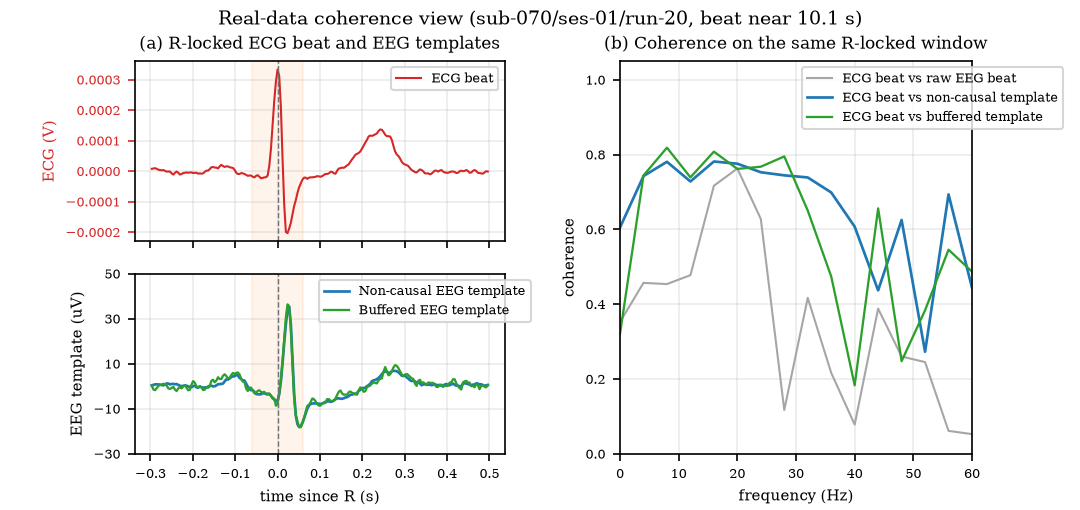
\includegraphics[width=\linewidth]{fig_real/fig_real_coherence_combined.png}
\caption{Real ear-EEG/ECG coherence. (a) Whole-record Welch estimate (0--60~Hz): indistinguishable
from zero across the spectrum. (b) Beat-synchronous estimate (8--20~Hz band), pooled over rolling
12-beat batches across a 10-minute recording (715 estimates): coherence stays low and stable even
under best-case R-locked alignment.}
\label{fig:coh}
\end{figure}

\begin{figure}[t]
\centering
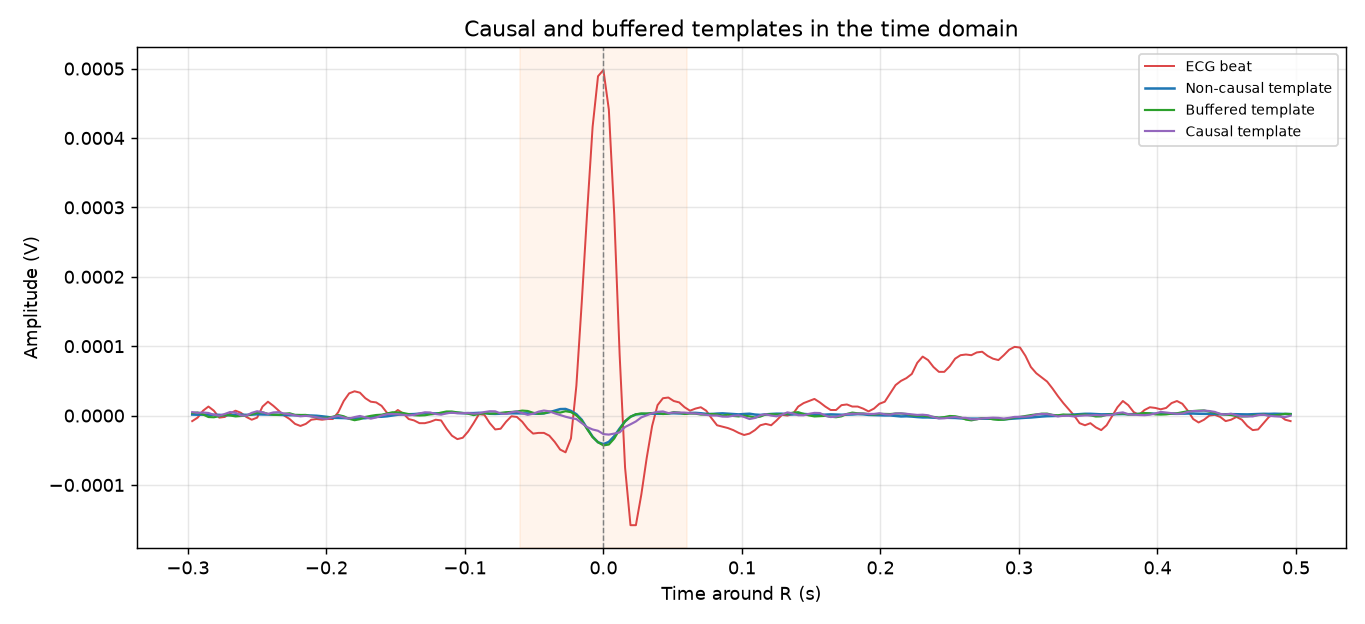
\includegraphics[width=0.85\linewidth]{fig_real/fig_real_causal_buffered.png}
\caption{Non-causal, buffered, and strict-causal templates learned from real ear-EEG (with one ECG
beat shown only for R-peak timing reference). A clear, repeatable R-locked deflection is recovered
despite the near-zero coherence of Fig.~\ref{fig:coh}. Buffered matches non-causal; the causal
(zero-latency) template's R-spike is measurably damped by RR-prediction error, confirming the
latency/suppression tradeoff of \S IV-B on physiological data.}
\label{fig:real_causal_buffered}
\end{figure}

\subsection{Semi-synthetic data}
The real-data evidence above has no ground truth $s(t)$, so we complement it with a semi-synthetic
protocol that provides exact-reference SNR metrics; the ILC-driven design validated qualitatively
above is here validated quantitatively. Following the semi-synthetic protocol common in EEG denoising \cite{zhang2021}, a low-CFA neural
surrogate (pink noise plus an amplitude-modulated 10~Hz alpha rhythm) provides ground truth $s(t)$. 
A synthetic ECG source $u(t)$ with RSA-modulated RR intervals is converted into a beat-locked 
artifact template with slow amplitude and morphology drift, then added at a controlled input SNR; 
one premature and one dropped beat are injected. This yields exact-reference metrics without manual 
labeling. Metrics: artifact SNR (steady state), spectral cardiac-peak reduction, and alpha 
preservation.

\subsection{Baselines}
Within the semi-synthetic protocol only (\S\ref{sec:realdata} shows why a reference-driven residual
stage cannot contribute on the real recording), we compare against (i)~a linear RLS/LMS
ECG-reference canceller \cite{widrow1975,haykin2014,sayed2008}; (ii)~an EKF/state-space canceller
\emph{[placeholder---to be added]} \cite{sameni2007}; and (iii)~low-channel ICA
\emph{[placeholder---to be added]} \cite{jung2000}, which is expected to degrade at $C<8$.

\subsection{Results}
Table~\ref{tab:results} reports steady-state artifact SNR for the main approaches, generated 
directly by the companion script to keep manuscript numbers synchronized with code. 
Fig.~\ref{fig:conv} shows single-pass online convergence for the three operating modes and the 
corresponding buffered-mode spectrum before and after cleaning. In single-pass online operation, 
buffered mode converges faster and to a higher final SNR than causal mode, consistent with the 
expected one-beat anchoring advantage. Spectrally, the cardiac comb is strongly reduced after 
cleaning while the 10~Hz alpha peak is preserved within about 10\%, an implicit 
heartbeat-evoked-potential safeguard \cite{park2019}. Ablations show that phase anchoring quality 
and mode selection (non-causal vs buffered vs strict-causal) dominate performance: buffered ILC is 
closest to non-causal performance, while strict-causal ILC is limited by RR prediction accuracy 
around sharp R-wave transitions.

\begin{figure}[t]
\centering

\includegraphics[width=0.85\linewidth]{fig1_convergence_spectrum.pdf}
\caption{(a) Online SNR convergence for the three modes (single causal pass). (b) Power spectrum 
before/after cleaning (buffered); shaded band marks the preserved 10~Hz alpha rhythm.}
\label{fig:conv}
\end{figure}

Fig.~\ref{fig:time} shows the time-domain cancellation over three consecutive beats in the 
converged regime. The synthetic reference $r(t)$ exhibits full PQRST morphology---P wave, QRS 
complex, and T wave---rather than a simplified sinusoidal surrogate, so the canceller must contend 
with a sharp, high-amplitude R deflection and a low-amplitude pre-R P wave. After processing, the 
cleaned EEG closely tracks the ground-truth neural signal $s(t)$: the R spike is suppressed by 
roughly an order of magnitude, the QRST tail is removed, and the residual P wave is attenuated, 
while the ongoing alpha oscillation is retained. This confirms that the phase-anchored template and 
residual canceller act on realistic cardiac morphology, not a reduced model.

\begin{figure}[t]
\centering

\includegraphics[width=0.85\linewidth]{fig2_timedomain.pdf}
\caption{Time-domain cancellation over three beats (converged, buffered mode). (a) Synthetic ECG 
reference $r(t)$ with full PQRST morphology; vertical lines mark detected R fiducials $t_k$. (b) 
Contaminated EEG $y(t)$, cleaned output, and ground-truth neural signal $s(t)$ over the same 
window.}
\label{fig:time}
\end{figure}

\end{document}
